\chapter[2025 April]{April 2025}

\section[2025/04/04]{Friday, 4 April 2025}
\label{sec:20250404}

Had massive issues and broke popos entirely. Had to reinstall but did Ubuntu 24.04.2 LTS

Not 100\% done with the setup but getting there.

This is also just to test the latex compiling using vscode.

Also got it compiled using the vimtex plugin (with lazyvim).


\section[2025/04/11]{Friday, 11 April 2025}
\label{sec:20250411}

Downloading the coco dataset for pose estimation. There are a number of places
you can get it but I downloaded it from the Kaggle website \href{https://www.kaggle.com/datasets/awsaf49/coco-2017-dataset?resource=download}{COCO2017 Download link}

Downloaded coco2017 and setup pipeline project.

Created a .venv in the root directory with requirements.txt so it can be reused for all the projects.

Work done in pipeline described in the README.md for example setting up pydantic settings to get the data directories as well as setting up matplotlib to display images.

Here is an example of a random image from the val2017 dataset with label

\begin{figure}[!ht]
	\centering
	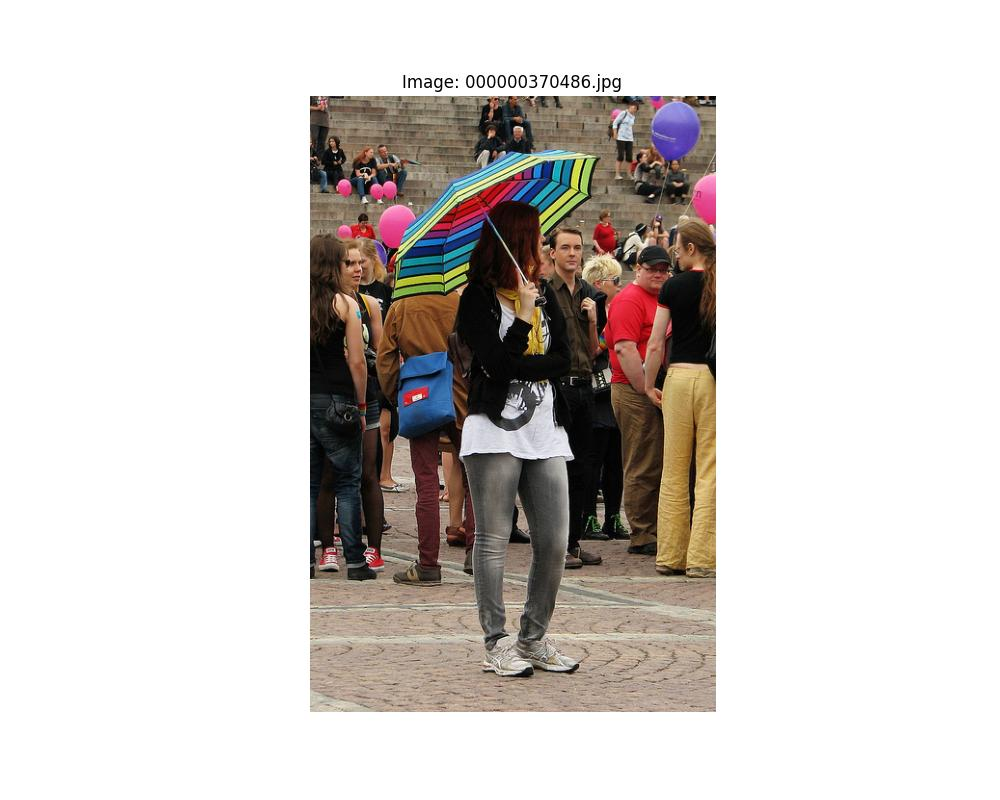
\includegraphics[width=1\linewidth]{figures/sample_000000370486.jpg}
	\caption{An example image from coco val2017 dataset (image 000000370486)}
	\label{fig:val2017_sample}
\end{figure}

Create a pytorch dataset using the coco dataset and pycocotools. Here you can select if you want training or validation and it will create the appropriate dataset

Use the dataset to create a basic dataloader. This isn't 100\% correct at this point due to the fact that the images are different sizes and I haven't scaled
them yet. For now I use a collate\_fn which groups images of the same size

\begin{lstlisting}[language=Python,title={How to do a basic dataloader in the pipeline project},label={code:basic_dataloader}]
import matplotlib
matplotlib.use('TkAgg')
import random
from torch.utils.data import DataLoader
from dataset import CocoKeypointsDataset

def custom_collate_fn(batch):
    # Group items by key
    result = {k: [item[k] for item in batch] for k in batch[0].keys()}
    return result

dataset = CocoKeypointsDataset(split='val')

print(f"Dataset size: {len(dataset)}")

batch_size = 4
dataloader = DataLoader(
    dataset, 
    batch_size=batch_size,
    shuffle=True,
    num_workers=2,
    collate_fn=custom_collate_fn
)

random_idx = random.randint(0, len(dataset) - 1)
output_path = dataset.visualize_item(random_idx)
print(f"Visualized sample at index {random_idx}")
print(f"Visualization saved to: {output_path}")

print("\nTesting DataLoader with batch size:", batch_size)
for batch in dataloader:
    images = batch['image']  # This is now a list of tensors
    keypoints_list = batch['keypoints']
    img_ids = batch['img_id']
    
    print(f"Number of images in batch: {len(images)}")
    
    # Print individual image shapes
    for i, img in enumerate(images):
        print(f"  Image {i} shape: {img.shape}")
    
    # Print people info
    for i, kps in enumerate(keypoints_list):
        print(f"  Image {i} (ID: {img_ids[i]}) has {len(kps)} people")
        
        for p, person_kps in enumerate(kps):
            visible_kps = (person_kps[:, 2] > 0).sum().item()
            print(f"    Person {p} has {visible_kps}/17 visible keypoints")
    
    break
\end{lstlisting}

The output will be something like this

\begin{lstlisting}[language={},title={Sample Output from Dataloader},label={code:dataloader_output}]
Testing DataLoader with batch size: 4
Number of images in batch: 4
  Image 0 shape: torch.Size([3, 399, 640])
  Image 1 shape: torch.Size([3, 422, 640])
  Image 2 shape: torch.Size([3, 500, 489])
  Image 3 shape: torch.Size([3, 612, 612])
  Image 0 (ID: 574520) has 1 people
    Person 0 has 13/17 visible keypoints
  Image 1 (ID: 161875) has 1 people
    Person 0 has 17/17 visible keypoints
  Image 2 (ID: 563281) has 1 people
    Person 0 has 12/17 visible keypoints
  Image 3 (ID: 16451) has 1 people
    Person 0 has 0/17 visible keypoints
\end{lstlisting}

Moved out the dataloader and setup a test.py file which does a basic test on it.

Basic depth estimation on the image using intel-isl/MiDaS (MiDaS\_small). This is fairly easy due to the fact I'm using
pytorch. I can just use the pretrained model

\begin{figure}[H]
	\centering
	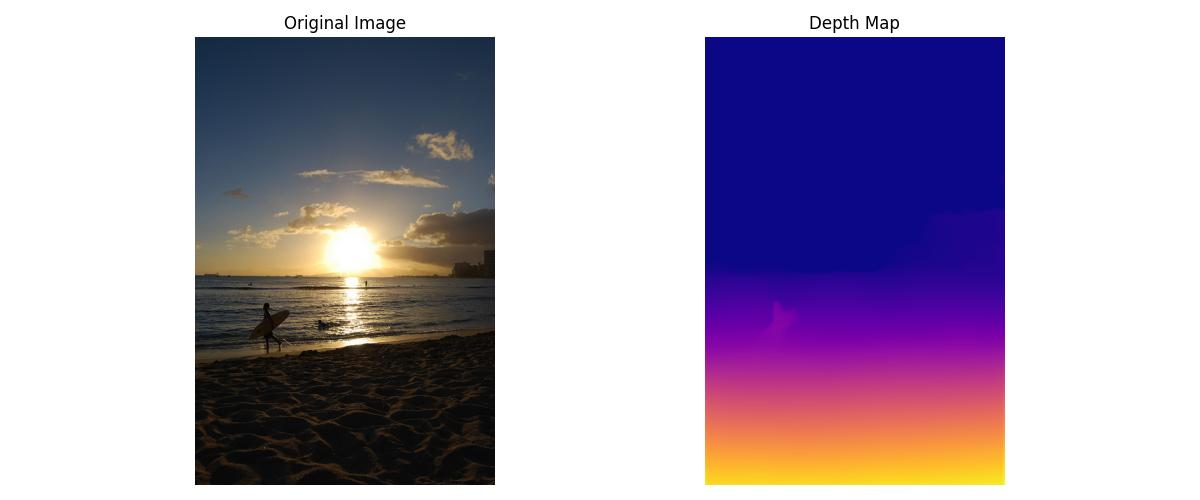
\includegraphics[width=1\linewidth]{figures/depth_estimation_304812.jpg}
	\caption{Example depth estimation on image 000000370486 from the val2017 dataset}
	\label{fig:val2017_depth_example}
\end{figure}

\begin{figure}[H]
	\centering
	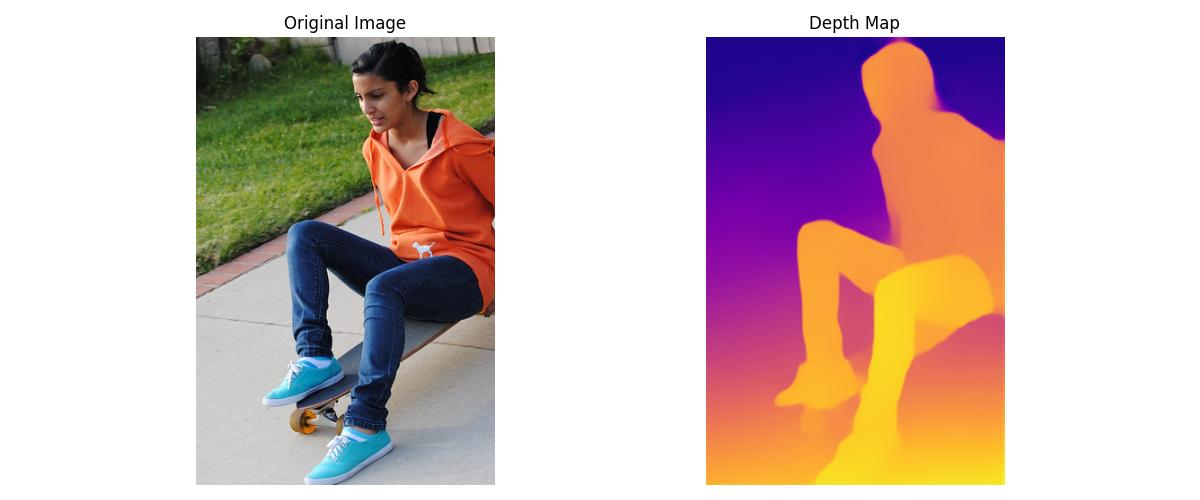
\includegraphics[width=1\linewidth]{figures/depth_estimation_108495.jpg}
	\caption{Example depth estimation on image 000000108495 from the val2017 dataset}
	\label{fig:val2017_depth_good_example}
\end{figure}

A good example of depth estimation is seen in \FigRef{fig:val2017_depth_good_example} where the person is in the foreground.

Again since I'm already using pytorch I can use a pretrained model for joint detection.

\begin{lstlisting}[language=Python,title={Resnet 50 pretrained pytorch model},label={code:resnet50_model}]
torchvision.models.detection.keypointrcnn_resnet50_fpn(pretrained=True)
\end{lstlisting}

\begin{figure}[H]
	\centering
	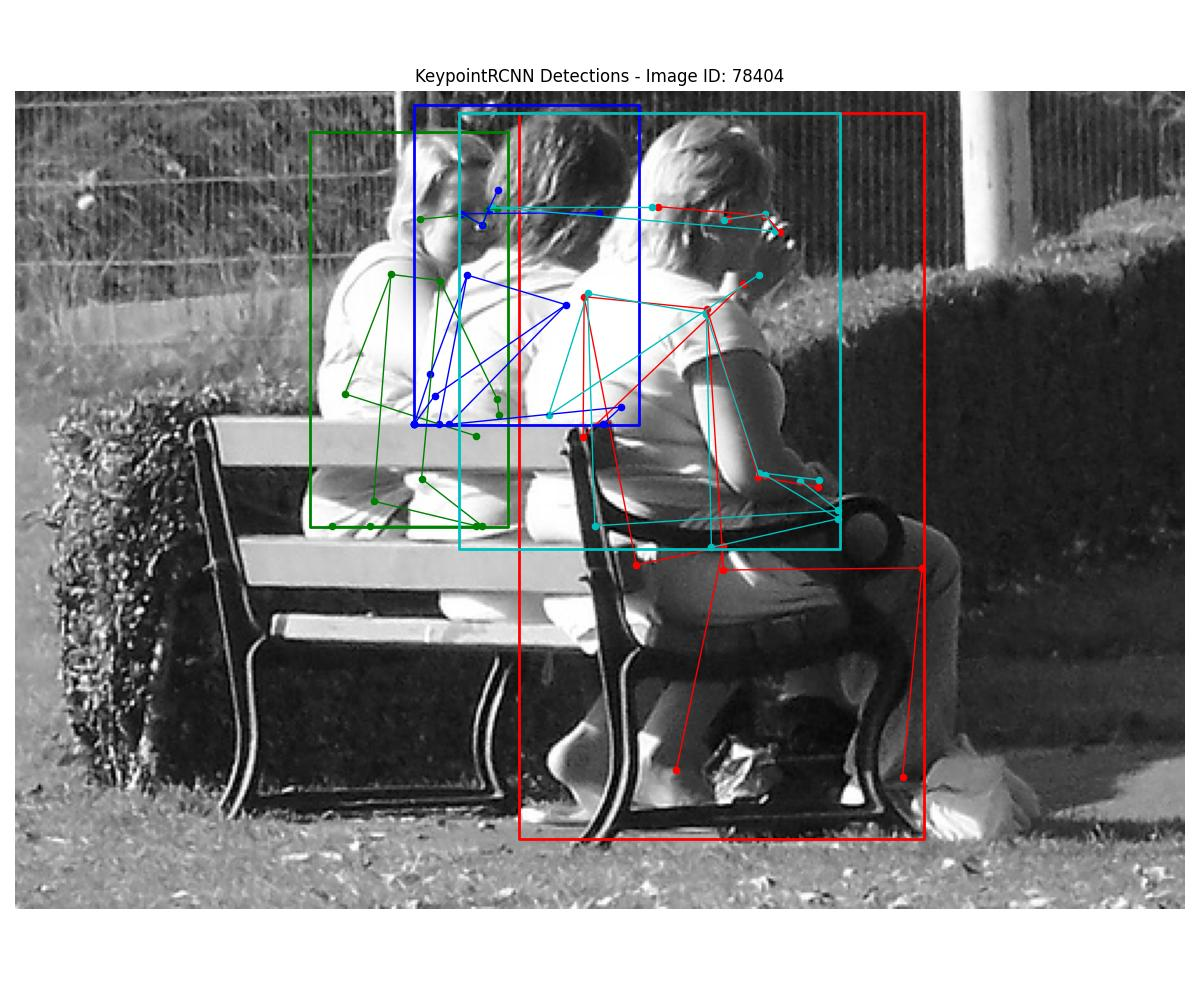
\includegraphics[width=0.48\linewidth]{figures/keypoint_rcnn_78404.jpg}\hfill
	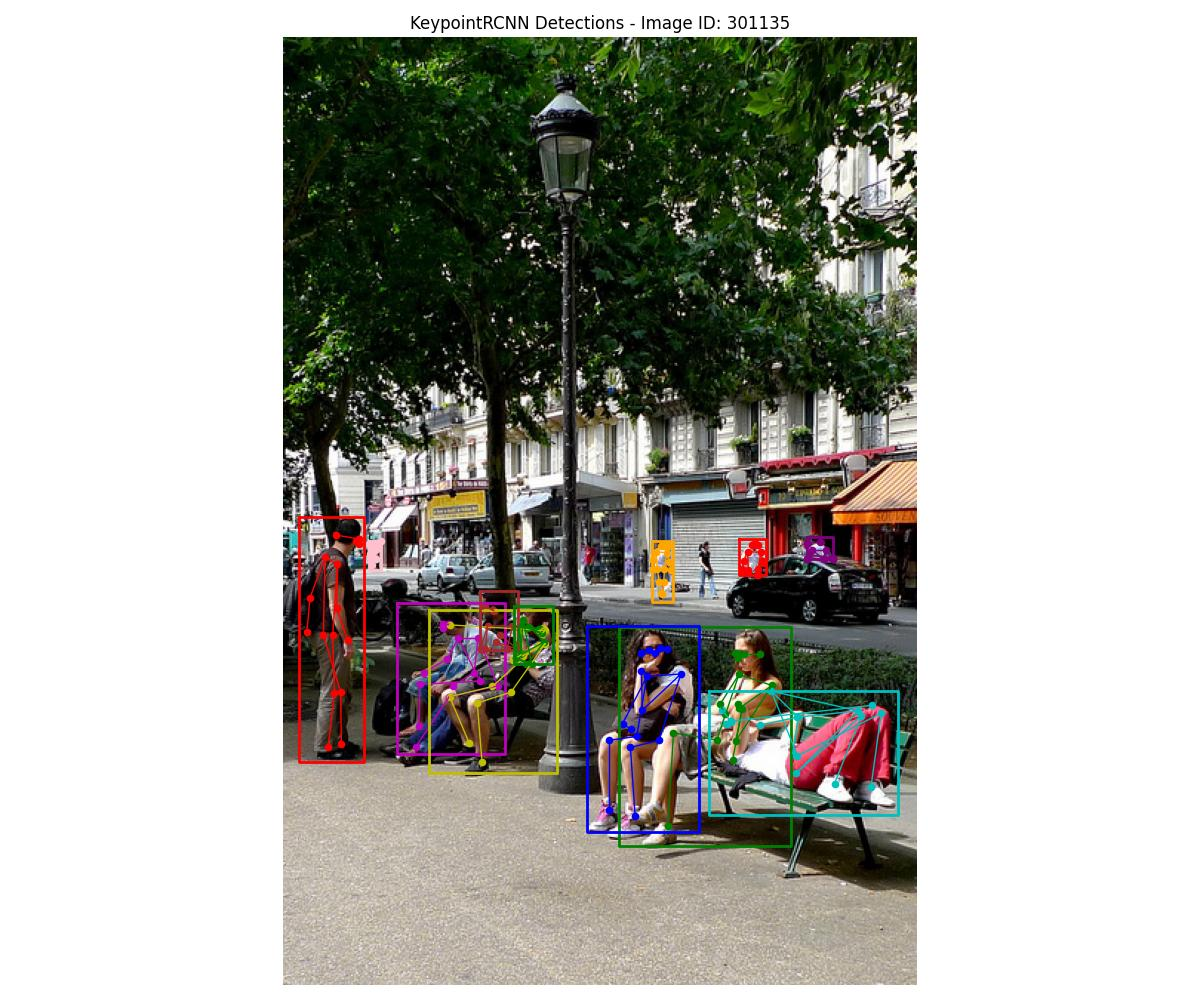
\includegraphics[width=0.48\linewidth]{figures/keypoint_rcnn_301135.jpg}\\[0.5em]
	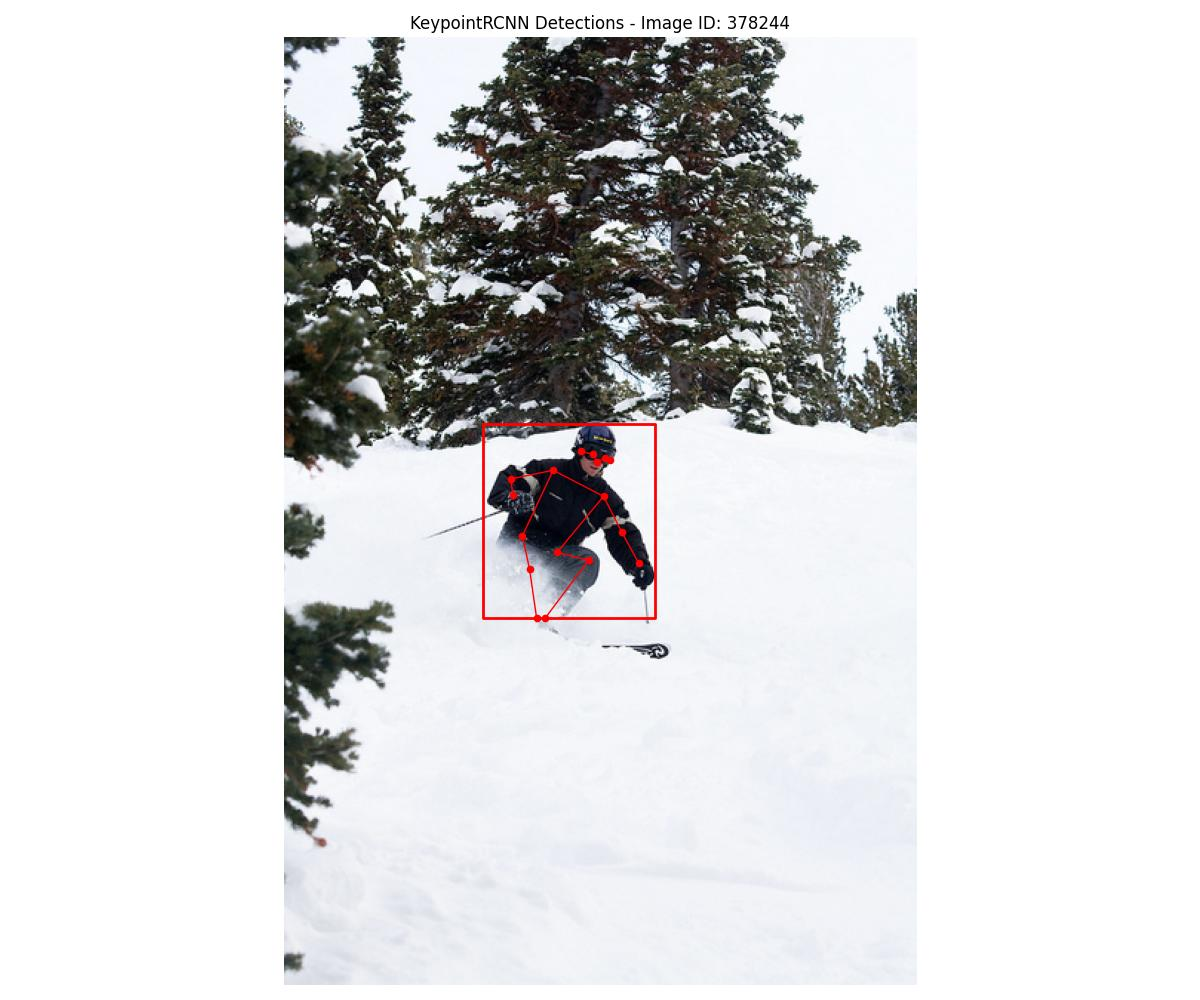
\includegraphics[width=0.48\linewidth]{figures/keypoint_rcnn_378244.jpg}\hfill
	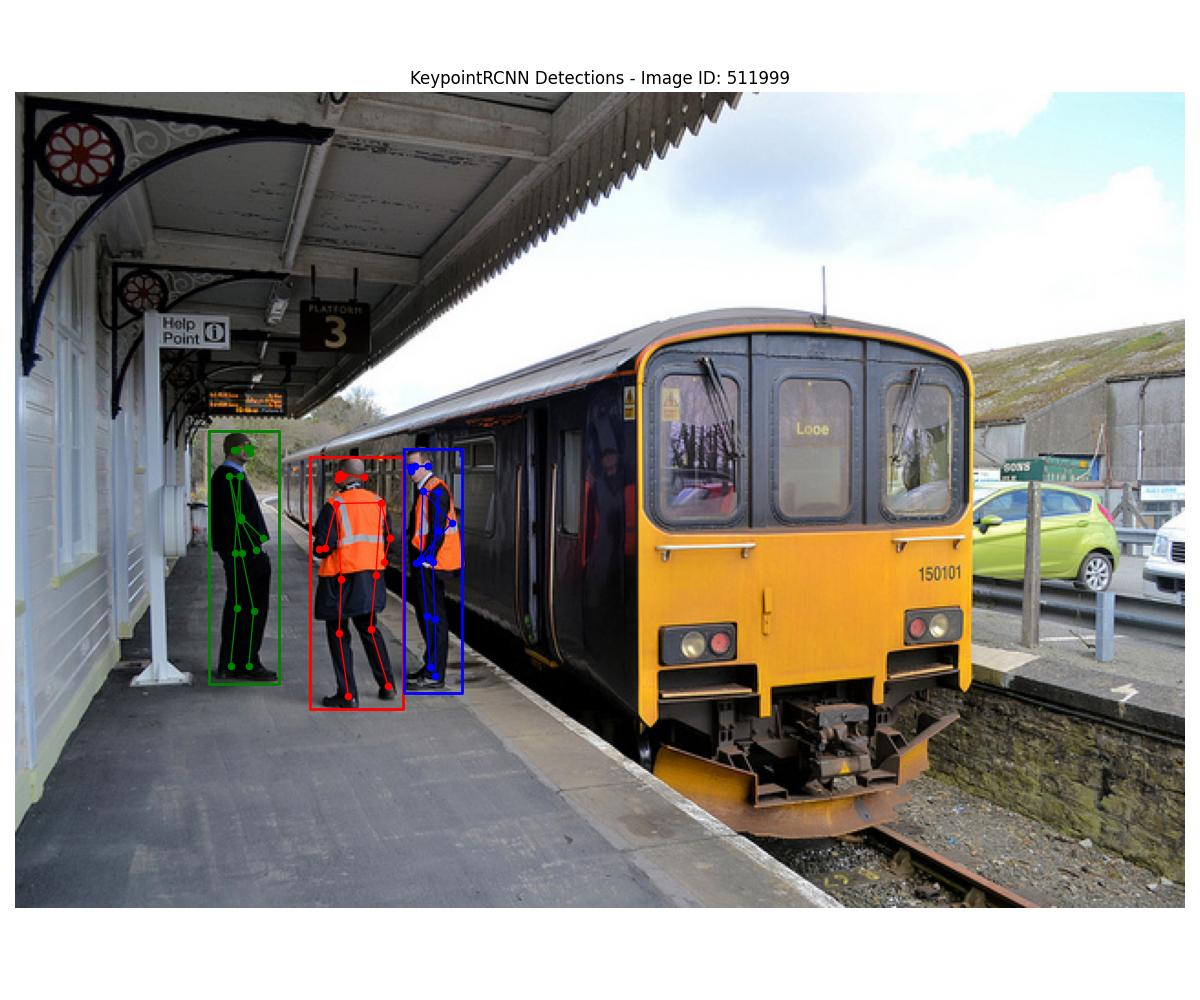
\includegraphics[width=0.48\linewidth]{figures/keypoint_rcnn_511999.jpg}
	\caption{Example joint detection using a ResNet-50 pretrained model on a number of randomly selected images.}
	\label{fig:val2017_resnet50}
\end{figure}


\section[2025/04/11]{Wednesday, 23 April 2025}
\label{sec:20250423}

This is a provisional plan to complete the masters

\begin{longtable}{@{} c c p{10.5cm} @{}}
\caption{Master's Project Timeline (25 Apr - 20 Nov 2025): Graph-Based Multiperson Pose Tracking}
\label{tab:masters-timeline}\\

\toprule
\textbf{Cycle} & \textbf{Dates} & \textbf{Key goals and deliverables} \\
\midrule
\endfirsthead

\toprule
\textbf{Cycle} & \textbf{Dates} & \textbf{Key goals and deliverables} \\
\midrule
\endhead

\midrule
\multicolumn{3}{r}{\small\itshape (continued on next page)}\\
\endfoot

\bottomrule
\endlastfoot
%
1  & 25 Apr - 8 May & • Finalise research questions and success metrics (mAP, MOTA, ID-F1)\\
   &                & • Dockerise a CUDA-enabled environment (PyTorch 2.x, TorchGeo, Weights \& Biases)\\
   &                & • Download COCO (or similar) and verify checksums\\
\midrule
2  & 9 - 22 May & • Build data-loading and augmentation pipeline for keypoints + instance masks\\
   &            & • Visual sanity-check: plot 100 annotated images to confirm loader correctness\\
   &            & • Outline baseline strategy (select off-the-shelf detector to integrate later)\\
\midrule
3  & 23 May - 5 Jun & • Integrate lightweight depth estimator (e.g., MiDaS) into the pipeline\\
   &                 & • Prototype \emph{depth-aware joint affinity}: encode 2-D offset and depth difference on edges\\
\midrule
4  & 6 - 19 Jun & • Design initial Graph Attention Network (nodes = joints; edges = affinity features)\\
   &             & • Implement PyTorch-Geometric \texttt{Data} objects and batching\\
\midrule
5  & 20 Jun - 3 Jul & • End-to-end draft: detector → depth → GAT → labelled poses\\
   &                 & • Small-scale training on a subset to debug convergence and memory use\\
\midrule
6  & 4 - 17 Jul & • Full-dataset training run; monitor loss and metrics automatically\\
   &            & • Hyper-parameter sweep (hidden dims, attention heads, depth-weight scaling)\\
\midrule
7  & 18 - 31 Jul & • Finalize training, comparisons, checking viability of the solution\\
   &             & • Make the model portable to implement in any pipeline\\
\midrule
8  & 1 - 14 Aug & • Implement first alternative tracker (e.g., transformer-based PoseTrack baseline)\\
   &            & • Run comparative evaluation with identical metric script\\
\midrule
9  & 15 - 28 Aug & • Implement second alternative and benchmark\\
   &             & • Aggregate results; generate summary tables and plots\\
\midrule
10 & 29 Aug - 11 Sep & • Begin writing paper for journal (as I understand it I need to publish to some academic journal)\\
   &            & • Choose a journal and get the template (or create one using latex)\\
\midrule
11 & 12 - 25 Sep & • Refine models if gaps appear during writing; lock final experimental protocol\\
   &             & • Complete first full draft for feedback\\
\midrule
12 & 26 Sep - 9 Oct & • Submit paper to chosen journal\\
   &                & • Start thesis: create scaffolding\\
\midrule
13 & 10 - 23 Oct & • Draft results, discussion, and conclusion chapters of thesis\\
   &             & • Address any comments received\\
\midrule
14 & 24 Oct - 6 Nov & • Assemble complete thesis draft; polish figures, references, and appendices\\
\midrule
15 & 7 - 20 Nov & • Incorporate feedback; final proof-read and submit thesis\\
\end{longtable}

\subsection{Graph Construction and Affinity-Aware Message Passing}
\label{sec:graph_construction}

A single image yields a set of \(N\) detected joints
\begin{equation}
\mathcal{J}
  =\bigl\{(x_i,\,y_i,\,d_i,\,c_i,\,t_i)\bigr\}_{i=1}^{N},
\label{eq:joint_set}
\end{equation}
where \((x_i,y_i)\) are image-plane coordinates,  
\(d_i\) the monocular depth estimate,  
\(c_i\in(0,1]\) the detection confidence,  
and \(t_i\in\{1,\dots,T\}\) the joint type
(e.g.\ \emph{left-wrist}, \emph{right-knee}).

\paragraph{Node features.}
Each joint is mapped to the node feature
\begin{equation}
\mathbf{n}_i
  =\bigl[x_i,\,y_i,\,d_i,\,c_i,\,\mathbf{e}_{t_i}\bigr]
  \in\mathbb{R}^{F},
\label{eq:node_feature}
\end{equation}
with \(\mathbf{e}_{t_i}\) a learnable embedding for the joint type.

\paragraph{Edge generation.}
Create an undirected edge \((i,j)\) whenever the Euclidean distance
\(r_{ij}=\lVert(x_i,y_i)-(x_j,y_j)\rVert_2\) is below a threshold \(\tau_r\).
Each edge carries an \emph{affinity feature} vector
\begin{equation}
\mathbf{a}_{ij}
  =\bigl[r_{ij},\;\lvert d_i-d_j\rvert,\;
          \cos\theta_{ij},\;
          c_i c_j\bigr]
  \in\mathbb{R}^{K},
\label{eq:affinity_vector}
\end{equation}
where \(\cos\theta_{ij}\) is the cosine of the angle between limb \((i,j)\)
and a reference limb (e.g.\ hip to joint \(j\)).

\paragraph{Affinity-aware attention.}
Given the graph \(G=(\mathcal{J},\mathcal{E})\),
a Graph Attention layer computes, for each edge,
\begin{equation}
\alpha_{ij}
  =\operatorname{softmax}_{j\in\mathcal{N}(i)}
     \Bigl(
       \mathrm{LeakyReLU}\bigl(
         \mathbf{a}^{\top}
         \bigl[
           W\,\mathbf{n}_i
           \,\Vert\,
           W\,\mathbf{n}_j
           \,\Vert\,
           W_e\,\mathbf{a}_{ij}
         \bigr]
       \bigr)
     \Bigr),
\label{eq:affinity_coef}
\end{equation}
where \(\mathbf{a}\) is a learnable vector,
\(W\in\mathbb{R}^{F'\!\times F}\) and
\(W_e\in\mathbb{R}^{F'\!\times K}\) are linear projections,
\(\Vert\) denotes concatenation,
and \(\mathcal{N}(i)\) is the neighbour set of node \(i\).

\paragraph{Node update.}
Nodes are updated via
\begin{equation}
\mathbf{h}_i
  =\sigma\!\left(
      \sum_{j\in\mathcal{N}(i)}
        \alpha_{ij}\,W_v\,\mathbf{n}_j
    \right),
\label{eq:node_update}
\end{equation}
with learnable \(W_v\) and activation \(\sigma(\cdot)\).

\paragraph{Person assignment.}
After \(L\) stacked attention layers, each node has representation
\(\mathbf{h}_i^{(L)}\).
A shallow classifier predicts whether an edge links joints of the
\emph{same} or \emph{different} people;
connected-component analysis on edges predicted “same-person”
produces the final joint-to-person assignments.